%\documentclass[12pt,t]{beamer}
\documentclass[xcolor=svgnames]{beamer}

%\usecolortheme[named=DarkBlue]{structure}

\usetheme{Boadilla}
%\usetheme[heigth=7mm]{Rochester}
%\usetheme{Rochester}
%\usetheme{Warsaw}
\usecolortheme{whale}
\useoutertheme{infolines}

\setbeamertemplate{blocks}[rounded][shadow=true]
%\setbeamertemplate{navigation symbols}{}
\usepackage[english]{babel}
\usepackage[utf8]{inputenc}
\usepackage{graphicx}
\usepackage{subfigure} 					% uso de many figures



\bibliographystyle{apalike}
% ------numbering frames-----------------------------------------%
%\newcommand*\oldmacro{}%
%\let\oldmacro\insertshorttitle%
%\renewcommand*\insertshorttitle{%
%	  \oldmacro\hfill%
%	  \insertframenumber\,/\,\inserttotalframenumber
%}
% ---------------------------------------------------------------%

% ------ References ---------------------------------------------%
\usepackage[absolute,overlay]{textpos}
\newenvironment{reference}[2]{%
  \begin{textblock*}{\textwidth}(#1,#2)
      \footnotesize\it\bgroup\color{red!50!black}}{\egroup\end{textblock*}}
% ---------------------------------------------------------------%

%\renewcommand{\figurename}{Figura}
%\renewcommand{\tablename}{Tabela}

% -------------------------------------------------------------- %
% Pacote necessário para subfiguras
\usepackage{multimedia, multirow}
\graphicspath{{./figures/}}
% -------------------------------------------------------------- %



%\title[II Charla Telecomunicaciones]{Software Libre aplicada en el Campo de las Telecomunicaciones}
%\subtitle{II Charlas de Telecomunicaciones ComSoc-UNI}
%\author[Christian Quispe]{Christian Quispe Quispe \\ \texttt{ christian.quispe@ieee.org}}
%\institute[UNI]{Universidad Nacional de Ingeniería}
%\date{29 de Noviembre del 2008}


\title[IEEE CAMAD 2012]
    {A Methodology to Define QoS and SLA Requirements in Service Choreographies}
\author[Alfonso Phocco-Diaz]
	{
		{\bf Authors} \\
		Victoriano Alfonso Phocco Diaz \\%\footnote{O aluno recebeu apoio financeiro do CNPq, processo 133147/2009-6} \\ [1ex]
		Daniel Macêdo Batista
		%{\bf Orientador} \\  Daniel Macêdo Batista 	\\
		%%{\bf Co-orientador} \\  Marco Dimas Gubitoso 	
	}
\institute[IME-USP]
	{Institute of Mathematics and Statistics \\
	 Departament of Computer Science \\	
	 University of São Paulo  \\  [1ex]
	 \texttt{alfonso7@ime.usp.br, batista@ime.usp.br}
	}
\date[September 2012]{September 17, 2012}



%%% Slides ---------------------------------
\begin{document}
%\pgfdeclareimage[width=180pt,height=20pt]{test}{images/header.jpg}
%\logo{\pgfuseimage{test}}

% --- the titlepage frame ------------------------------------------%
\begin{frame}[plain]
\titlepage
\end{frame}

\section*{Agenda}
    \begin{frame}{Agenda}
        \tableofcontents
    \end{frame}

% ------------------------------------------------------------------%
\AtBeginSection[]
{
	\begin{frame}<beamer>
		\frametitle{}
		\tableofcontents[currentsection]
	\end{frame}
}

% ------------------------------------------------------------------%
% ------------------------------------------------------------------%
% --- Introduction ---------------------------------------------------%
\section{Introduction}

    \begin{frame}
        \begin{block}{Objetives }\vspace{-.3\baselineskip}
        	\begin{itemize}
                  \item
		  \item  
            \end{itemize}
        \end{block}
    \end{frame}

    \begin{frame}{Problem}
    	\begin{itemize}
          \item <1-> Planning of resources before/during development of choreography.
          \item <2->\textbf{Contratos probabilísticos} refletem melhor o comportamento dinâmico dos \textbf{atributos de QoS}.
    	\end{itemize}
    \end{frame}

  \begin{frame}{Justification}
    	\begin{itemize}
          \item <1-> Planning of resources before/during development of choreography.
          \item <2->\textbf{QoS} is a important factor for adaptation, selection, otimization, service composition into SOC.
          
    	\end{itemize}
  \end{frame}



% ------------------------------------------------------------------%
% ------------------------------------------------------------------%
% --- Basic Concepts ---------------------------------------------------%
\section{Basic Concepts}
  \begin{frame}{Web Service}
    	\begin{itemize}
          \item <1-> .
          
    	\end{itemize}
  \end{frame}

  \begin{frame}{Service Orchestration}

  \end{frame}


%----- Coreografia de Serviços -----
    \begin{frame}{What is service choreography?}
      \begin{figure}[!h]
         \centering
         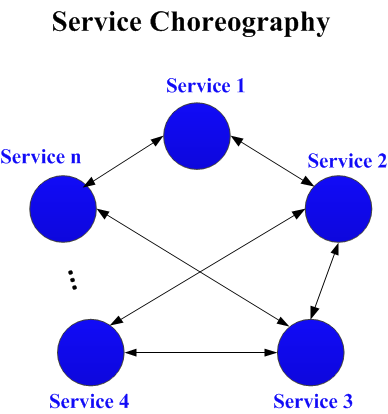
\includegraphics[width=0.5\textwidth]{figures/ChoreographyA.png}
         \caption{Service Choreography }
          %\begin{reference}{4mm}{85mm}
           %         Casanova, Henri and Legrand, Arnaud and Quinson, Martin,
            %	{SimGrid: a Generic Framework for Large-Scale Distributed Experiments},
            %	IEEE Computer Society, 2008.
            %\end{reference}
      \end{figure}	

    \end{frame}



%----- Qualidade de Serviços -----
    %\begin{frame}{Qualidade de Serviço}
        %\begin{itemize}
          %\item Quality of Service : QoS.
          %\item \textbf{Funcionalidade/serviço} = quais operações o sistema executa.
         %       \begin{itemize}
        %            \item Exemplo: compra de passagens de avião.
       %         \end{itemize}

      %    \item \textbf{QoS/característica não funcional} = como o sistema executa esses serviços.
     %           \begin{itemize}
    %                \item Exemplo: O tempo médio de resposta é 2 segundos.
   %             \end{itemize}
  %        \item Importante em várias áreas de SOC.
 %       \end{itemize}
%    \end{frame}

%---------- Qualidade de Serviço ---------
    \begin{frame}{Quality of Service}
      \begin{figure}[!h]
          \centering
          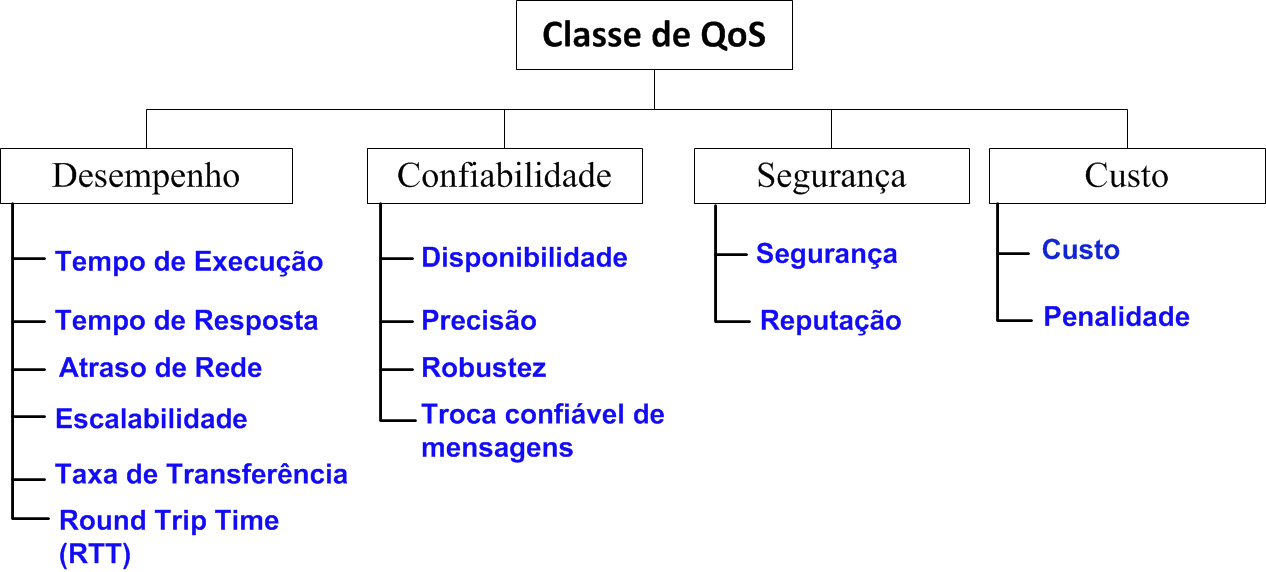
\includegraphics[width=1.0\textwidth]{QoSTaxonomy.png}
          \caption{Taxonomia de atributos de QoS \cite{Rosenberg2006}}
          %\label{fig:QoST_SLA_Mapping_Transformation}
      \end{figure}	
      
      \tiny{
        \begin{thebibliography}{2}
         %         \beamertemplatearticlebibitems
           \beamertemplatearticlebibitems
          \bibitem[Rosenberg et al.,2006]{Rosenberg2006}
            Rosenberg F, Platzer C, Dustdar S. {\em Bootstrapping Performance and Dependability Attributes of Web Services}.
            IEEE International Conference on Web Services (ICWS’06). 2006:205-212.
            %\newblock {\em Bootstrapping Performance and Dependability Attributes of Web Services}.
            %\newblock IEEE International Conference on Web Services (ICWS’06). 2006:205-212.
       \end{thebibliography}
      }
    \end{frame}


  \begin{frame}{Process Choreography}
   
  \end{frame}

  \begin{frame}{BPMN and Choreography}
   
  \end{frame}

  \begin{frame}{Example}
   
  \end{frame}



% ------------------------------------------------------------------%
% ------------------------------------------------------------------%
% -------------------- Methodology ---------------------------------%
\section{Methodology}
  \begin{frame}{Description}
  
  \end{frame}


  \begin{frame}{Choreography Formalization}
   
  \end{frame}

  
  \begin{frame}{QoS Model}
   
  \end{frame}


  \begin{frame}{Mapping BPMN to Petri Net (I)}
   
  \end{frame}


  \begin{frame}{Mapping BPMN to Petri Net (II)}
   
  \end{frame}

  
  \begin{frame}{Mapping Algorithm }
   
  \end{frame}
  


  

% ------------------------------------------------------------------%
% ------------------------------------------------------------------%
% -------------------- Performance Evaluation ----------------------%
\section{Performance Evaluation}
  \begin{frame}{Scenario}
  
  \end{frame}


  \begin{frame}{Mapping}
   
  \end{frame}


  \begin{frame}{ Configuration}
   
  \end{frame}


  \begin{frame}{ Simulation}
   
  \end{frame}



  \begin{frame}{ Results}
   
  \end{frame}





%---------- Conclusions ----------------
\section{Conclusions and Future Works}
   \begin{frame}{Conclusions}
       \begin{itemize}
         \item <1->  We have prosposed a Nobel methodology to aid define QoS and SLA requirements in service Choreography.
	 \item <2->  
       \end{itemize}
   \end{frame}

  \begin{frame}{Future Works}
       \begin{itemize}
         \item <1->  .
	 \item <2->  
       \end{itemize}
   \end{frame}



%\bibliographystyle{apalike}% citação bibliográfica alpha
%\def\newblock{}
 %       \bibliography{slides}
 %   \end{thebibliography}
%\end{frame}


%--------- fim ----------
    \begin{frame}%{\textbf{Thanks!}}
        \begin{block}{}\vspace{-.3\baselineskip}
        	Thanks so much!
        \end{block}

    \end{frame}




\end{document}